
\subsection{Kommandozeile}

\subsubsection{Aufgaben}
Die Kommandozeile stellt dem Anwender die Möglichkeit zur Verfügung, Befehle in einer einfachen Scriptsprache in ein Textfeld einzugeben und diese per Klick auf einen Button auszuführen. Es soll möglich sein eine Reihe an Befehlen einzugeben, die anschließend vom Roboter, in der angegebenen Reihenfolge, ausgeführt werden. Weiters soll der Benutzer in einer Konsole über Fehler beziehungsweise die erfolgreiche Übersetzung der Befehle informiert werden.

\subsubsection{Aufbau}
Die Benutzeroberfläche für diesen Anwendungszweck besteht aus zwei Textfeldern, wobei nur eines editierbar und somit zur Eingabe vom Befehlen geeignet ist. Das andere Textfeld stellt die Konsole dar und dient der Ausgabe von Informationen während der Kompilierung des eingegebenen Scripts. \\
Bei Klick auf den entsprechenden Button, analysiert die Klasse CommandParser den eingegebenen Text auf richtige Syntax. Fehlen Semikolons oder Klammern so wird eine InvalidSyntaxException, mit einer passenden Meldung ausgelöst. Diese Meldung wird in der Konsole angezeigt und informiert den Benutzer über Fehler im Code. Ist die Syntax des Befehls richtig, so wird dieser, gemeinsam mit den Parameterwerten, der CommandBuilder-Klasse übergeben.\\
Diese Klasse ermittelt um welches Command es sich genau handelt und versucht ein entsprechend Objekt aus der Edubot-API zu erzeugen. Wird bei der Generierung eine fehlerhafte Parameteranzahl beziehungsweise ungültige Werte entdeckt, so wird eine InvalidParameterException mit Details über den Fehler ausgelöst und in der Konsole angezeigt. Das erzeugte Objekt wird einer Liste mit Befehlen hinzugefügt, welche nach erfolgreicher Kompilierung an die Edubot-Klasse übergeben wird.

\subsubsection{Bedienung der Oberfläche}

\begin{figure}[H]
  \centering
  \begin{minipage}[t]{12 cm}
  	\centering
  	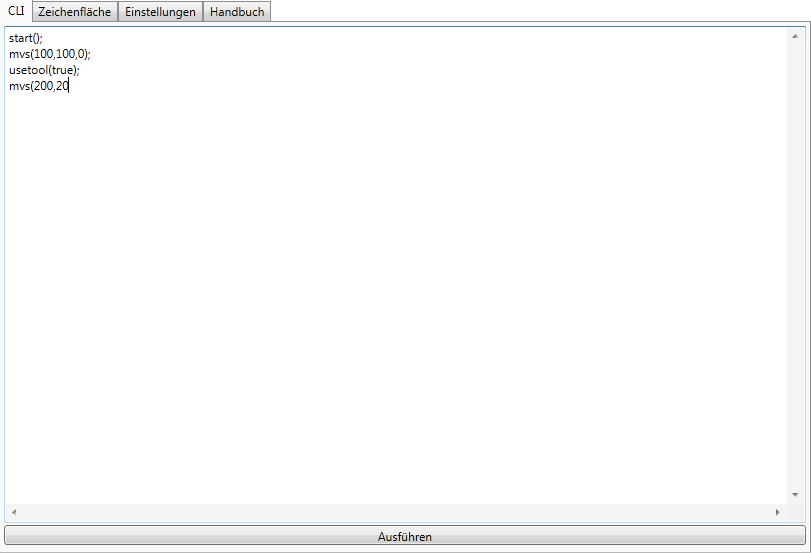
\includegraphics[width=12cm]{images/CLI} 
    \caption{Die Kommandozeile}
  \end{minipage}
\end{figure}

Die Bedienung der Kommandozeile ist für den Anwender relativ simpel. Um zum Einggabefeld für den Code zu gelangen muss lediglich auf das Tab "'Kommandozeile"' geklickt werden. Anschließend erscheint auch schon der entsprechende Editor, in den nun beliebige Befehle eingegeben werden können. Durch einen Klick auf das "Play"-Symbol in der Werkzeugleiste werden die Eingabe kompiliert und anschließend ausgeführt. Je nach Anzahl und Art der registrierten Adapter kann die Dauer der Ausführung variieren.

\subsubsection{Umsetzung}
Durch die, von der API zur Verfügung gestellte, Kommando-Infrastruktur war die Umsetzung dieser Aufgabe relativ einfach. Die größte Herausforderung war das Entwickeln der CommandParser-Klasse, da diese eine gültige Syntax gewährleisten muss. Ist die Syntax gültig so werden die extrahierten Informationen der CommandBuilder-Klasse übergeben, welche daraus entsprechende ICommand-Objekte erzeugt.\\
\\
\textbf{CommandParser}\\
Die CommandParser-Klasse übernimmt die Syntax-Validierung des eingegebenen Texts und gibt erhaltene Informationen über Befehlsart und Parameterwerte an die CommandBuilder-Klasse weiter. Die Klasse verfügt nur über eine statische Methode und zwar:
\begin{itemize}
\item \textbf{Parse}\\
Dieser Methode übernimmt als Parameter einen String mit dem zu kompilierenden Text und liefert als Ergebnis eine Liste mit ICommand-Objekten. 
Bei Aufruf von CommandParser.Parse wird zuerst eine neue Liste für die generierten ICommands erzeugt und der mitgegebenen Text mit Hilfe der Split-Methode der String Klasse und "';"' als Trennzeichen aufgeteilt. Anschließend wird durch das entstandene Array iteriert und jeder Eintrag analysiert. Im ersten Schritt wird mit Hilfe der Contain-Methode geprüft ob der String ein "'("'- und ein "')"'-Zeichen enthält. Falls dem nicht so ist, so wird eine InvalidSyntaxException mit entsprechender Meldung ausgelöst.\\
Im nächsten Schritt des Analyseprozesses wird der Name des eingegebenen Befehls mit Hilfe der Substring-Methode extrahiert, welcher sich zwischen dem ersten Zeichen und dem ersten Auftreten eines "'("'-Zeichens befinden sollte. Die Parameter eines Befehls sollten sich zwischen den Klammern befinden und werden erneut mit Hilfe der Substring-Methode herausgefiltert. Anschließend wird noch die Split-Operation mit einem "',"' als Trennzeichen ausgeführt um die einzelnen Parameterwerte in einem String-Array zu erhalten.\\
Die erhaltenen Informationen werden anschließend der statischen BuildCommand-Methode der CommandBuilder-Klasse übergeben, welcher deraus ein ICommand-Objekt generiert. Dieses Objekt wird der, im ersten Schritt erzeugten Liste, angehängt, die bei erfolgreicher Ausführung der Methode als Ergebnis zurückgeliefert wird.
\end{itemize}
\textbf{CommandBuilder}\\
Da sichergestellt werden muss, das es sich bei den übergebenen Parametern um gültige Werte handelt, müssen sie zuvor validiert werden. Bei erfolgreicher Validierung muss daraus ein entsprechendes ICommand-Objekt erzeugt werden, das der Execute-Methode der Edubot-Klasse letzten Endes mitgegeben werden kann. Diese Aufgaben werden vom sogenannten CommandBuilder unter Verwendung folgender Methoden erfüllt:
\begin{itemize}
\item \textbf{BuildCommand}\\
Die Methode BuildCommand übernimmt als Parameter einen String mit dem Befehlsnamen und ein String-Array mit den dazugehörigen Parametern. Innerhalb der Methode wird mit einer switch-Kontrollstruktur geprüft ob es einen Befehl mit diesem Namen gibt. Tritt dieser Fall ein, so wird eine der später erläuterten Methoden des CommandBuilders ausgeführt und ein passendes ICommand-Objekt zurückgegeben, andernfalls wird eine UnknownCommandException ausgelöst. 
\item \textbf{BuildStartupCommand}\\
Die Methode BuildStartupCommand wird aufgerufen wenn es sich beim eingegebenen Befehl um "'start"' handelt. Sie übernimmt als Parameter ein String-Array mit Parametern. Da das StartupCommand keine Argumente übernimmt wird geprüft ob die Länge des Arrays null ist. Trifft dieser Fall zu, so wird ein neues Objekt vom Typ StartupCommand erzeugt und zurückgegeben, andernfalls wird eine InvalidParameterException mit einer entsprechenden Nachricht ausgelöst.
\item \textbf{BuildShutdownCommand}\\
Die Methode BuildShutdownCommand wird aufgerufen wenn es sich beim eingegebenen Befehl um "'shutdown"' handelt. Sie übernimmt als Parameter ein String-Array mit Parametern. Auch das ShutdownCommand übernimmt keine Argumente, weshalb hier ebenfalls geprüft wird ob die Länge des Arrays null ist. Trifft dieser Fall zu, so wird ein neues Objekt vom Typ ShutdownCommand erzeugt und zurückgegeben, andernfalls wird eine InvalidParameterException mit einer entsprechenden Nachricht ausgelöst.
\item \textbf{BuildMVSCommand}\\
Die Methode BuildMVSCommand wird aufgerufen wenn es sich beim eingegebenen Befehl um "'mvs"' handelt. Sie übernimmt als Parameter ein String-Array mit Parametern. Ein MVSCommand benötigt die X-, Y- und Z-Koordinate des Zielpunkts, weshalb im ersten Schritt geprüft wird ob die Länge des Arrays genau drei ist.\\
Anschließend wird mit Hilfe der int.TryParse-Methode versucht die String-Werte in Integer-Werte zu konvertieren. Schlägt die Konvertierung bei einem der mitgegebenen Werte fehl oder entspricht die Länge des Arrays nicht der Vorgabe, so wird eine InvalidParameterException mit einer entsprechenden Nachricht ausgelöst.
\item \textbf{BuildMVCCommand}\\
Die Methode BuildMVCCommand wird aufgerufen wenn es sich beim eingegebenen Befehl um "'mvc"' handelt. Sie übernimmt als Parameter ein String-Array mit Parametern. Ein MVCCommand benötigt die X-, Y- und Z-Koordinate des Ziel- und des Mittelpunkts, weshalb im ersten Schritt geprüft wird ob die Länge des Arrays genau sechs ist. \\
Anschließend wird mit Hilfe der int.TryParse-Methode versucht die String-Werte in Integer-Werte zu konvertieren. Schlägt die Konvertierung bei einem der mitgegebenen Werte fehl oder entspricht die Länge des Arrays nicht der Vorgabe, so wird eine InvalidParameterException mit einer entsprechenden Nachricht ausgelöst.
\item \textbf{BuildUseToolCommand}\\
Die Methode BuildUseToolCommand wird aufgerufen wenn es sich beim eingegebenen Befehl um "'usetool"' handelt. Sie übernimmt als Parameter ein String-Array mit Parametern. Ein UseToolCommand benötigt als Parameter einen Wert vom Typ Boolean, welcher angibt ob das Werkzeug aktiviert oder deaktivert werden soll. Auch hier wird zuerst überprüft ob die Länge des Arrays genau eins beträgt.\\
Anschließend wird versucht den Wert mit Hilfe der bool.TryParse-Methode in einen boolschen Wert zu konvertieren. Schlägt die Konvertierung fehl oder entspricht die Länge des Arrays nicht der Vorgabe, so wird eine InvalidParameterException mit einer entsprechenden Nachricht ausgelöst.
\end{itemize}

